\documentclass{article}

\usepackage[final]{nips_2017}

\usepackage[utf8]{inputenc} % allow utf-8 input
\usepackage[T1]{fontenc}    % use 8-bit T1 fonts
\usepackage{hyperref}       % hyperlinks
\usepackage{url}            % simple URL typesetting
\usepackage{booktabs}       % professional-quality tables
\usepackage{amsfonts}       % blackboard math symbols
\usepackage{nicefrac}       % compact symbols for 1/2, etc.
\usepackage{microtype}      % microtypography
\usepackage{graphicx}
\usepackage{amsmath}
\usepackage{amssymb}
\usepackage{listings}
\usepackage{courier}
\usepackage{multirow}

\lstset{basicstyle=\ttfamily\footnotesize,breaklines=true}
\title{CSE 253 Progress Report -- Fashion Image Generation with ICGAN  }

\author{
  Fanjin Zeng \\
  Computer Science and Engineering\\
  University of Califorina, San Diego\\
  \texttt{f1zeng@ucsd.edu} \\
   \And
   Xinyue Ou \\
   Computer Science and Engineering\\
   University of Califorina, San Diego \\
   \texttt{x1ou@ucsd.edu} \\
   \And
   He Qin \\
   Computer Science and Engineering\\
   University of Califorina, San Diego \\
   \texttt{h9qin@ucsd.edu} \\
   \And
   Yuhan Chen \\
   Eletrical and Computer Engineering\\
   University of Califorina, San Diego \\
   \texttt{yuc143@ucsd.edu} \\
}

\begin{document}

\maketitle
\section{Topic Migration}
In our proposal, we planned to explore DCGAN(Deep Convolutional Generative Adversarial Network) using different dataset. Now we decide to make our project more application specific. We want to realize fashion clothes generation and synthesis using IcGAN (Invertible Conditional Generative Adversarial Network) [1]. In [1], IcGAN is used to do face synthesis, that is given an input face picture, the network is able to generate a target facial picture with specified characteristics, such as wearing glasses, having bang or being bald. In our application, we want to apply the same idea to DeepFasion dataset[3], which consists of more than 800,000 fashion images. 

\begin{figure}[h]
\centering
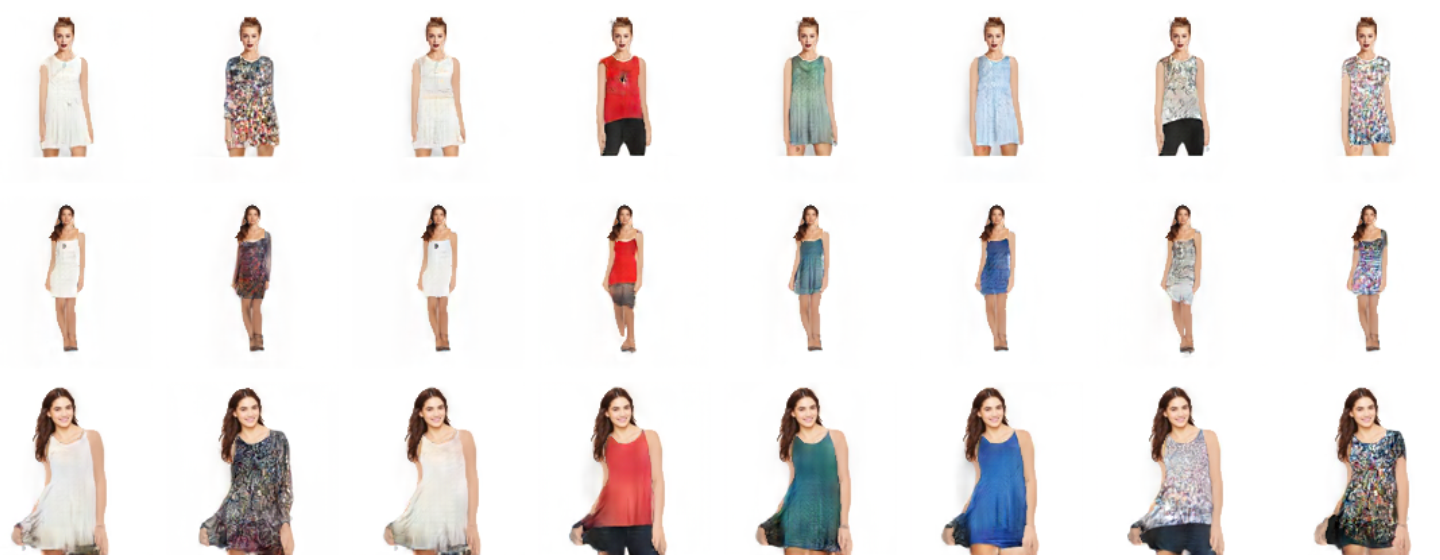
\includegraphics[width=1\linewidth]{pics/clothes.png}
\caption{Synthesizing different fashion clothes given one model pose image}
\label{fig:clothes}
\end{figure}





\section{Progress}
Currently we have built the proposed IcGAN model[1] using TensorFlow. The architecture composes of two encoders, one encoding the latent representation z and the attribute information y. We will train the encoder $E_z$ along with the cGAN and train encoder $E_y$ separately. To generate a modified image, we will apply variation on the attribute vector to have different conditions such that we can generate a image with the same structure as the input image but different flavors.

\begin{figure}[h]
\centering
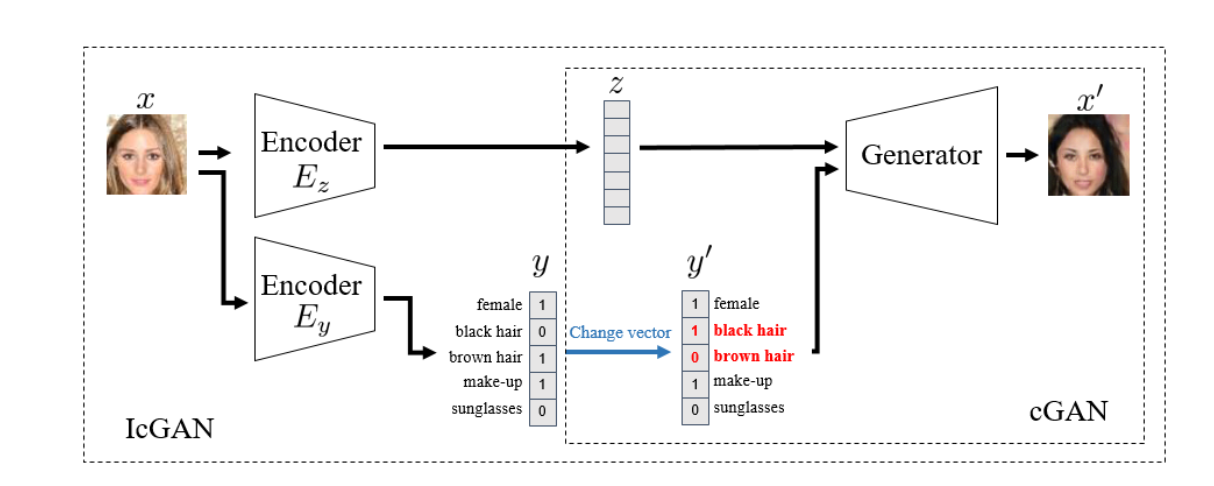
\includegraphics[width=0.7\linewidth]{pics/scheme.png}
\caption{Scheme of a trained IcGAN}
\label{fig:scheme}
\end{figure}

Moreover, we preprocessed DeepFashion dataset[3] by applying the bounding boxes of the clothes and scaling the images to better accommodate our application. 
  \begin{figure}[h]
  \centering
  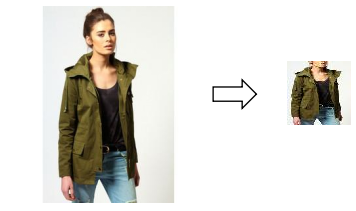
\includegraphics[width=0.7\linewidth]{pics/preprocess.png}
  \caption{Preprocess image by applying bounding box and resizing to 64x64}
  \label{fig:preprocess}
  \end{figure}
\section{Reference}
[1] Perarnau, Guim, et al. "Invertible conditional gans for image editing." arXiv preprint arXiv:1611.06355 (2016).

[2] Zhu, Shizhan, et al. "Be your own prada: Fashion synthesis with structural coherence." arXiv preprint arXiv:1710.07346 (2017).

[3] Liu, Ziwei, et al. "Deepfashion: Powering robust clothes recognition and retrieval with rich annotations." Proceedings of the IEEE Conference on Computer Vision and Pattern Recognition. 2016.


\end{document}